% Intended LaTeX compiler: pdflatex
\documentclass{scrartcl}
    \usepackage[utf8]{inputenc}
    \usepackage[dvipdfmx]{color}
    \usepackage[backend=biber,bibencoding=utf8]{biblatex}
    \usepackage{url}
    \usepackage{indentfirst}
    \usepackage[normalem]{ulem}
    \usepackage[dvipdfmx]{hyperref}
    \usepackage{longtable}
    \usepackage{minted}
    \usepackage{fancyvrb}
    \usepackage[dvipdfmx]{graphicx}
    \bibliography{reference}
\author{江畑 拓哉(201611350)、栗本真太郎(201511366)、畑中 智之(201611402)}
\date{}
\title{seis-ml-api中間レポート}
\begin{document}

\maketitle
\tableofcontents

\section{情報特別演習概要}
\label{sec:org9f80ab5}
本演習は江畑、栗本、畑中の3名により実施する。それぞれ演習を進め、最終的に大規模データベースを用いた機械学習API(seis-ml-api)を作成することが目標である。\\

\subsection{演習範囲に関して}
\label{sec:org40df129}
Table1に示す範囲を演習し、その成果を組み合わせることでseis-ml-apiの作成を目指す。\\

\begin{table}[htbp]
\caption{演習範囲に関して}
\centering
\begin{tabular}{|c|c|c|}
\hline
氏名 & 分野 & 内容\\
\hline
江畑 & データベースと機械学習の統合 & 大規模データを利用した機械学習の作成\\
\hline
栗本 & 機械学習 & 機械学習モデルの調整\\
\hline
畑中 & データベース & 大規模データベースの作成\\

\hline
\end{tabular}
\end{table}

\subsection{seis-ml-api概要}
\label{sec:orgd312151}
seis-ml-apiは、機械学習を提供するWeb APIである。大規模データベースを採用する。seis-ml-apiのフローをFigure.1に示す。\\

\begin{figure}[htbp]
\centering
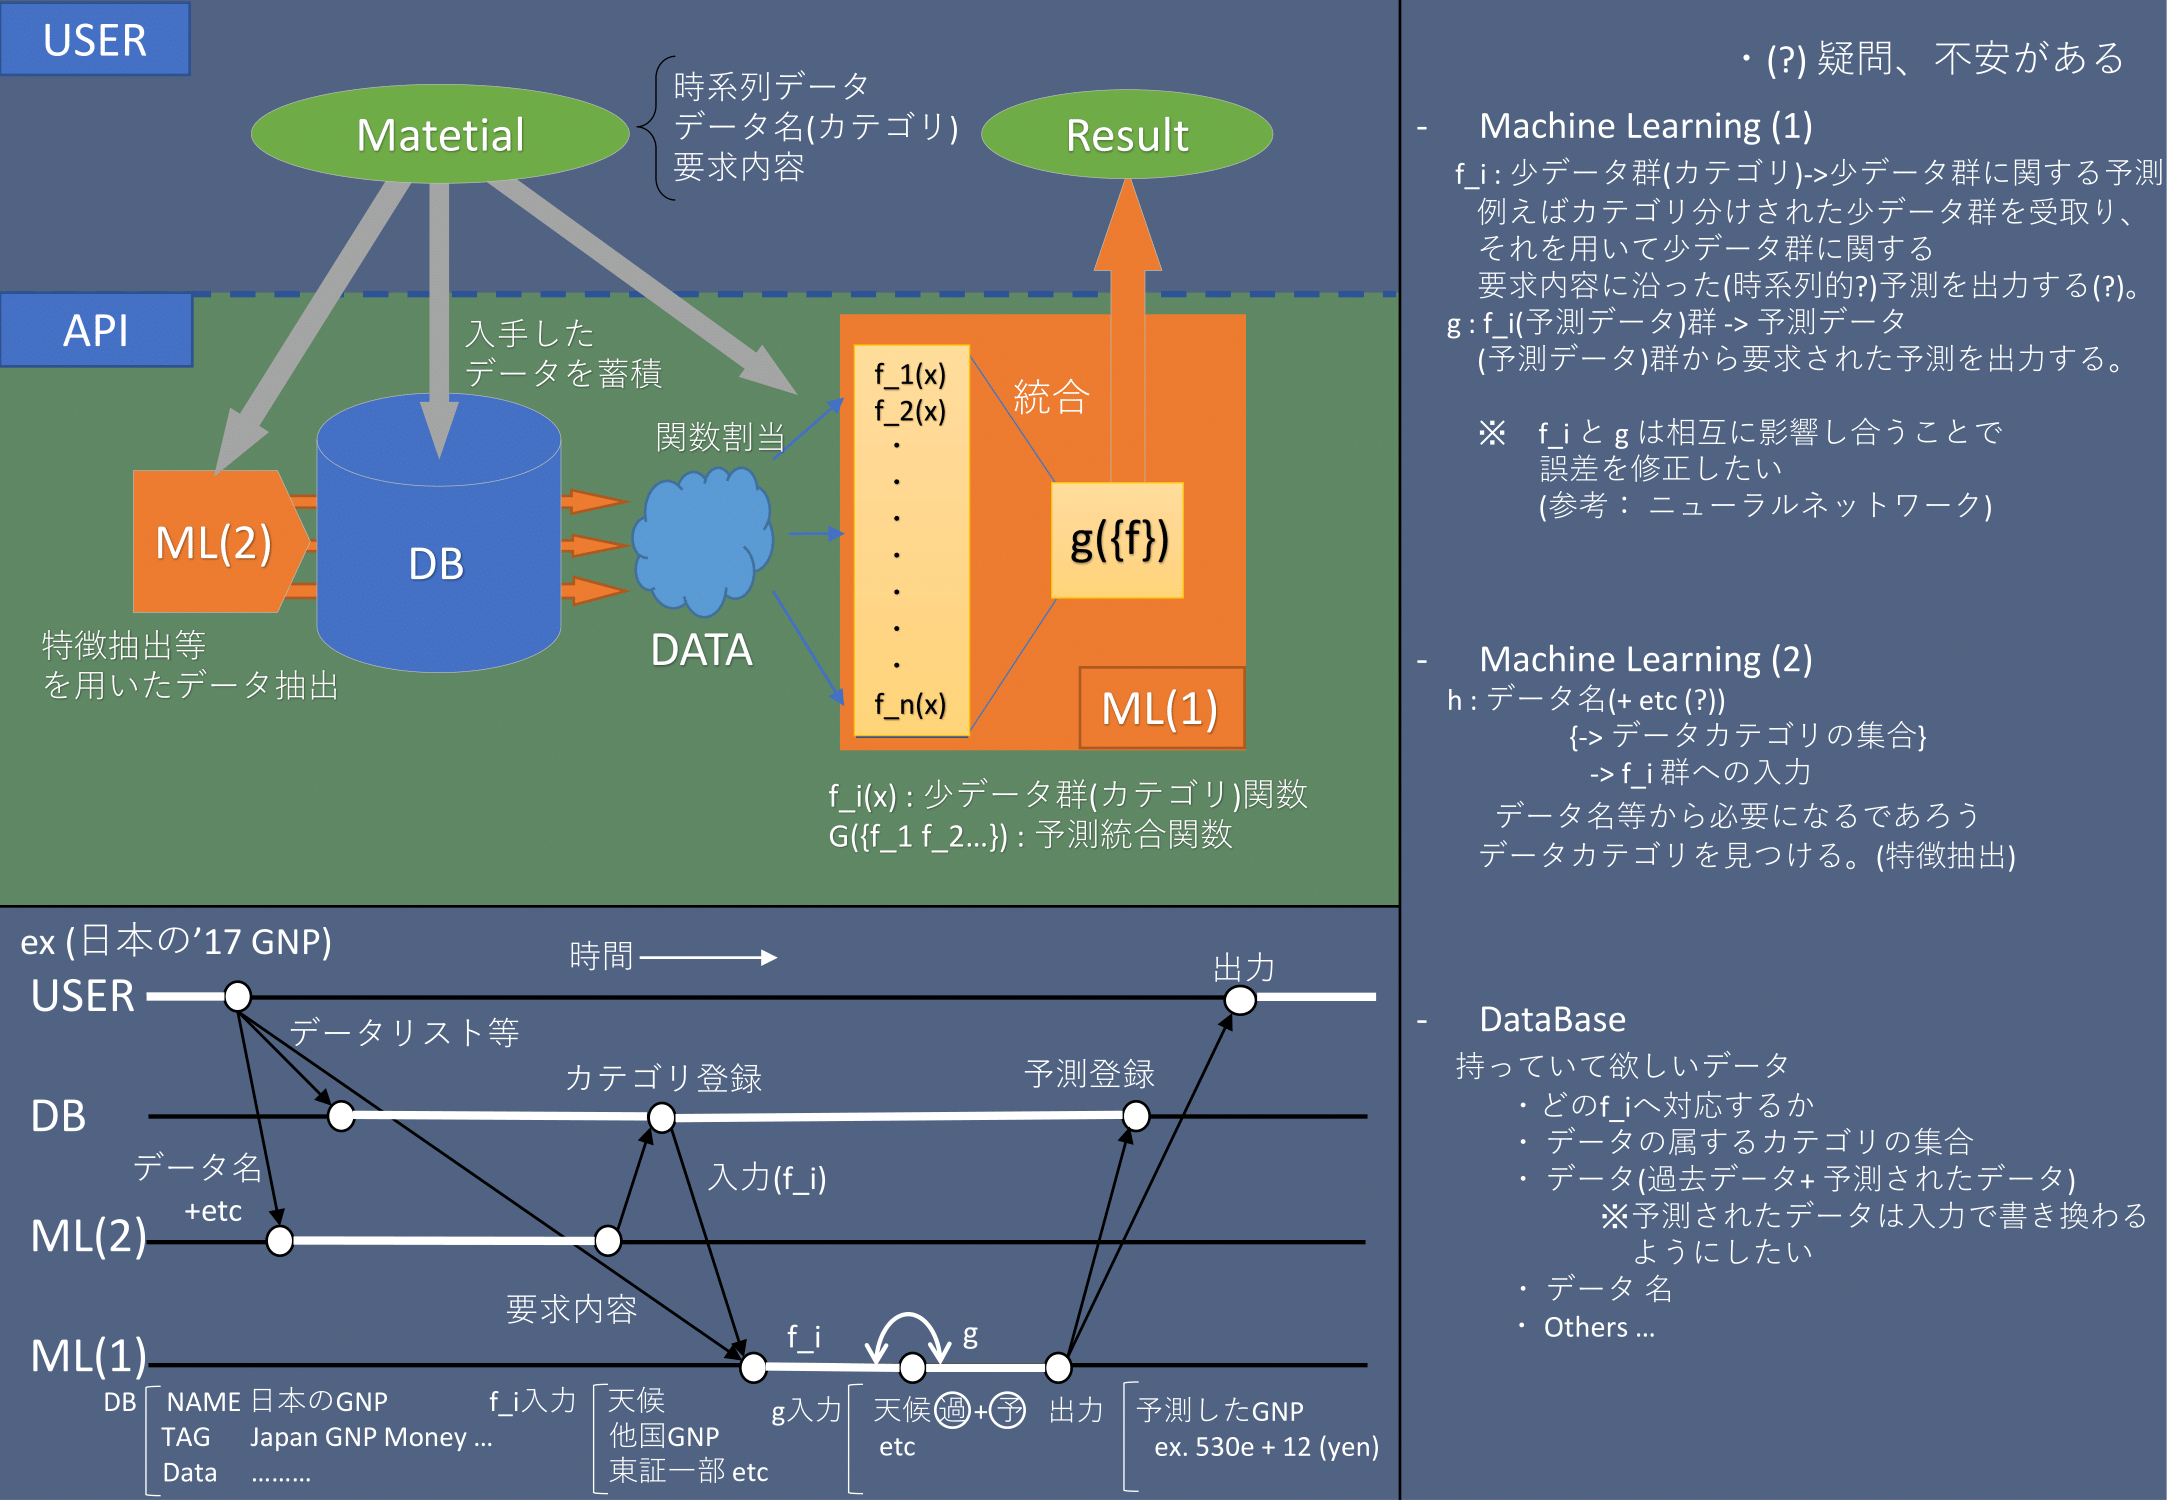
\includegraphics[width=15cm]{./idea-0-1.png}
\caption{seis-ml-apiのフロー}
\end{figure}

ユーザはAPIに自分の持っているデータを登録する。APIは、APIに登録されているデータを用いて機械学習処理を行い、その結果をユーザに返す。\\

\subsection{実験に用いるデータ}
\label{sec:org3a61408}
以下のデータをデータベースに登録し、実験段階においても用いたいと考えている。データの相関を求める関係上、これらの入手元から日本国内の経済についてのデータを集めたいと考えている。\\

\begin{itemize}
\item Quandl\\
ほとんどすべてのデータはここで手に入る。ただし、長期間のデータは乏しいようである。主には、ここから得た株価データを用いて分析を行う予定である。\\
\item google finance\\
日本のデータをcsv形式で入手することは困難だが、海外のデータは容易に手に入る。\\
\item 総務省統計データ\\
めぼしいデータは少ないが、ゼロではないため活用していきたい。\\
\end{itemize}

\section{それぞれの進捗について}
\label{sec:org4e0996c}
\begin{itemize}
\item 江畑\\
機械学習アルゴリズムの策定を行った。また Java 、Python 、Clojure での HBase の利用方法について学習した。\\
\item 栗本\\
「機械学習」の履修及び関連書籍の学習を行った。また、主専攻実験「ヒューマンセンシング」の自主実験において、サポートベクターマシンを用いた簡易画像分類器を作成した。\\
\item 畑中\\
HBase 、Hadoop を用いて疑似分散環境を構築した。また、JavaからHBaseにアクセスする方法を、実際にプログラムを動作させて確認した。\\
\end{itemize}


\section{今後の演習について}
\label{sec:orgf289936}
\begin{itemize}
\item 江畑\\
\end{itemize}
策定した機械学習のモデルを実際のコードに実現する作業とHBaseに入力されたデータを送るAPIを作成する。\\
\begin{itemize}
\item 栗本\\
\end{itemize}
機械学習モデルの理解を深め、Pythonによるデータ分析に慣れ、より良いモデル調整が可能なように学習していきたいと考えている。\\
\begin{itemize}
\item 畑中\\
\end{itemize}
完全分散環境を構築して、HBaseの性能テストを行いたいと考えている。\\

\end{document}